% ===========================================================================
% v3 §4 — GUIDES AND SENSORS ALONG THE BURST (~2 pp; figures F2 + F3)
% Draft r2 (2026-09-03): numbers-verifier fixes — typed outcomes (INCONCLUSIVE / structural exclusion; the v2 word
% "non-identifiable" exists nowhere in the repo), edge stamps as the audit record defines them (3.92 kT vs band edge,
% 20 keV trust floor), "at least four" query forms, strict >6 for strong, lessons in 5 of 10 step skills.
% Draft r1 (2026-09-03), architecture block with §3 r4 and §7 r1 (decision 20: one gate for §3+§4+§7).
% Absorbs from v2: "The campaign loop" steps paragraph (v2:264-288, re-ordered to the OFFICIAL ledger
% 0b,0,1-9 — PI ruling 2026-08-30 — and step 8 = nuFnu panels), "Inside the fitting step" (v2:312-340) with
% v2's fig:fitstep TikZ as F3 (outline: "v2 Fig. 2 unchanged"; r2 changed two boxes: typed outcomes / INCONCLUSIVE and
% strict >6; r3 after the F3 delta gate: multistarts wording (thermal restarts are LRT-gated, scripts/10 ~1293-1303),
% 'vs. best simpler ancestor' (NESTED_PARENTS, not the simplest menu model), arrows anchored at .north), the fan-out/verifier-gates
% paragraph (v2:359-371). P0 freeze + three-way attribution -> §6; K-clean/freeze -> §5 (one pointer each).
% Tone per decisions 18/19: describe what runs and what checks it; PROPOSED once; no claims.
% Figure F2 = paper_agentic/figures/fig_F2_lifecycle_guides_sensors (gated; shas in figures/GATE_LEDGER.md).
% F3 TikZ uses v2's preamble styles (box, dec, arr, lab) — present at splice time.
% Model-count wording follows the engine (6 base + 2 free-smoothness + 16 high-energy = 24), not v2's 4+5+15.
% ===========================================================================
\section{Guides and Sensors Along the Burst} \label{sec:sensors}

Section~\ref{sec:harness} took the harness apart by job. This section
follows one burst through it in time. The unit of work is one burst walked
through eleven ledger steps, and at every step the harness does two things
besides run the step: it steers the model before the step with
\emph{guides}, the skill document, the checklist, and the standing
contracts that apply, and it checks the result after the step with
\emph{sensors}, some of them code and some of them fresh-context roles.
Figure~\ref{fig:lifecycle} draws the ledger with the guides on the left and
the sensors on the right; grey sensors are code, white ones are model
judgement, and the diamond between them is the human gate that every step
passes before the next begins.

\begin{figure*}[t]
\centering
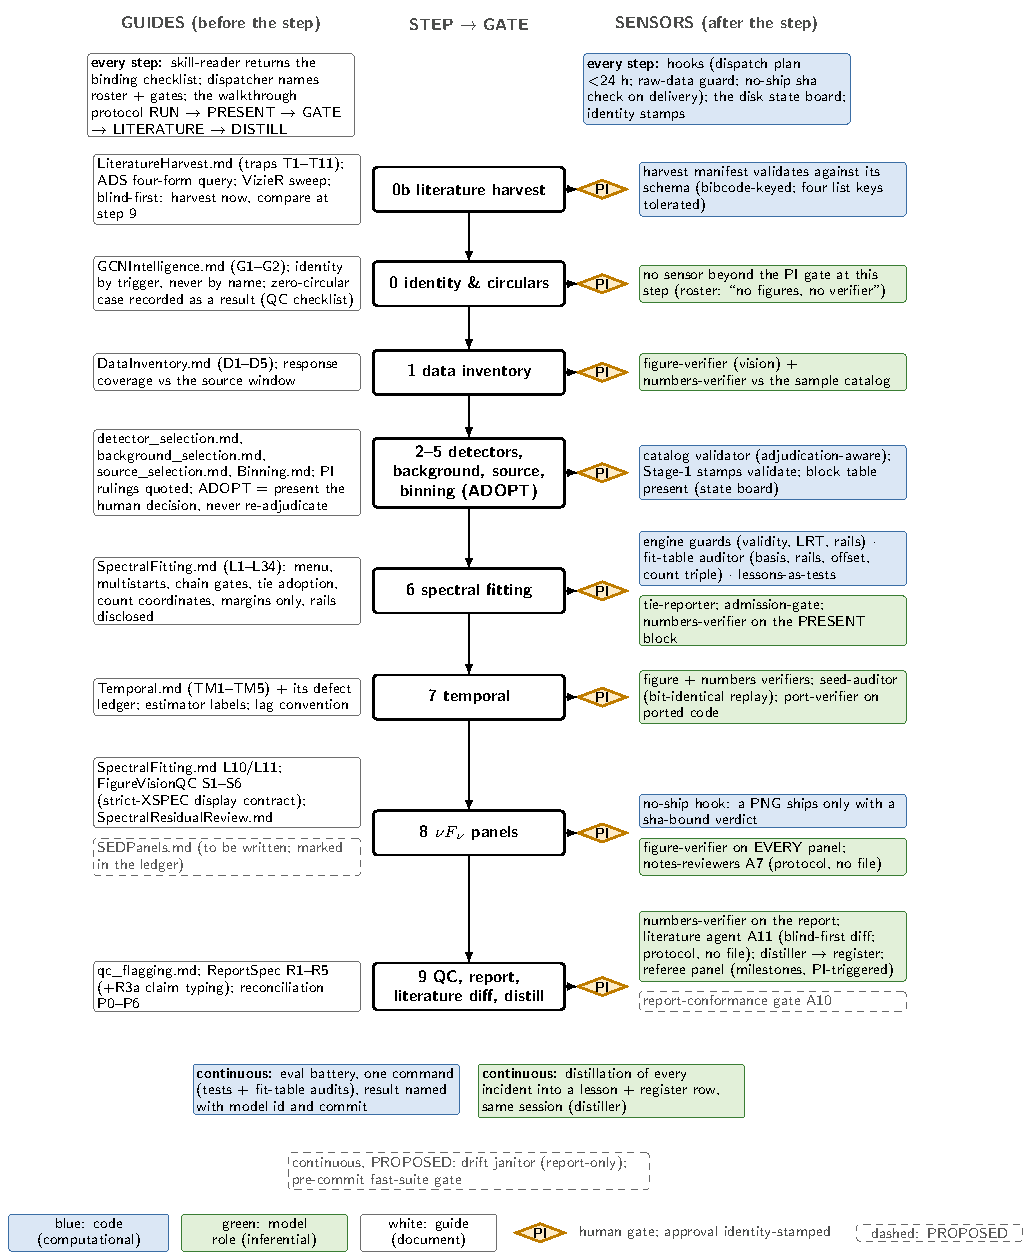
\includegraphics[width=0.92\textwidth]{figures/fig_F2_lifecycle_guides_sensors.pdf}
\caption{The per-burst lifecycle with its guides and sensors. Centre: the
eleven ledger steps, top to bottom, each followed by the human gate.
Left: the guides that steer each step before it runs, chiefly the step's
skill document with its numbered lessons and the standing contracts in the
human's words. Right: the sensors that check each step after it runs, grey
where the check is code (tests, hooks, the fit-table auditor, schema
validation) and white where it is a fresh-context role (figure, numbers,
seed, port verifiers; the tie reporter; the admission gate). Below the
ledger, the checks that run continuously. Dashed items are proposed.}
\label{fig:lifecycle}
\end{figure*}

\subsection{The eleven steps} \label{sec:steps}

The ledger begins before the data. The \emph{literature harvest} (step 0b)
finds and fetches every refereed paper that analysed the burst, using at
least four query forms (the GRB name, the trigger name, the day fraction, the trigger
number), preferring the version of record, and recording each harvested
value with its conventions: which peak-energy definition, which sign
convention for the lag, which energy band, which time interval on whose
clock, which detectors. The harvest is taken early and compared late; the
comparison itself waits for step 9, after our own numbers are frozen
(\S\ref{sec:doctrine}). The \emph{identity and circulars} step (0)
resolves which burst this actually is, since same-day triggers exist, and
reads every real-time circular; a burst with no circular is recorded as a
result, not as a gap. The \emph{data inventory} (1) verifies that the
downloaded data can support the analysis: file versions, response-matrix
time coverage against the source window, and detector geometry, including
the check that no well-placed detector is occulted by the spacecraft, a
failure invisible to pointing angles alone. The three \emph{selection}
steps (2--4: detectors, background windows, source window) are decided by a
human in a purpose-built interface or by a vision-capable role, and either
way recorded with a stamp naming the decision-maker and the mode; downstream
the pipeline treats those stamps as immutable inputs, and the walkthrough
presents the recorded decision rather than re-adjudicating it. The
\emph{adaptive binning} step (5) derives Bayesian-block time bins from the
reference detector and merges them to a significance floor. \emph{Spectral
fitting} (6), where most of the bounded agency lives, has its own
subsection below. The \emph{temporal} step (7) measures the duration, the
minimum variability timescale, and the spectral lag from the same approved
selections, with the estimator named on every value and the lag sign
convention stated. The \emph{spectral-energy panels} (8) render every bin
under the display semantics of the standard X-ray fitting package and are
read residual by residual. \emph{Quality control} (9) assembles the report,
runs the literature comparison, and closes the burst with a typed verdict
and named flags. A bin in which no model passes the validity gate is
declared inconclusive by the engine, and a burst whose response does not
cover its source window is excluded structurally; both are recorded,
\emph{successful} outcomes. The workflow is forbidden to keep adjusting an
analysis until it manufactures a preference.

The guides are the same kind of object at every step: the step's skill
document, read end to end by the skill reader before the step opens, with
its criteria, its checklist, and, where the step has accumulated them, its
numbered lessons; for the selection
steps the human's rulings quoted verbatim; for the figure and report steps
the standing contracts. The sensors differ by step because the artifacts
differ. A harvest manifest is validated against its schema. An inventory
figure passes the figure verifier and its numbers are recomputed against
the sample catalog. A stamped selection is validated by the catalog
validator, and the state board records the block table before fitting may
start. A fit table passes the engine's own guards, the fit-table auditor
(the argmin, the rails, the tie set, the count coordinates), the
lessons-as-tests, and, on presentation, the tie reporter and the numbers
verifier. A temporal product passes the figure and numbers verifiers, the
seed auditor, which replays any stochastic product from its recorded seed,
and the port verifier where code was ported. A panel cannot reach the human
unless its hash is in the verification ledger, and every panel is read by
the figure verifier. The report passes the numbers verifier and the
blind-first literature comparison; a report-conformance gate that would
check the report against its contract as code is specified and proposed.
Beneath the ledger two checks run continuously: the evaluation battery,
one command that runs the test suite and the fit-table auditor over every
promoted table and records, with its result, the model identity it was
given and the commit,
and the distillation of every incident into a lesson and a register row
in the session that produced it (\S\ref{sec:learning}).

\subsection{Inside the fitting step} \label{sec:fitstep}

The fitting engine confronts each time bin with twenty-four spectral
models: six base models, two free-smoothness variants, and sixteen
high-energy extensions (Fig.~\ref{fig:fitstep}). Three rules govern what
the numbers may mean. First, \emph{inclusion is gated on data quality,
never on detection significance}: every detector band with usable data and
a valid response enters the joint fit, because conditioning inclusion on
significance manufactures spurious detections in exactly the bursts where a
band fluctuated upward. Second, \emph{every model family receives multistarts}: unconditional for
the continua and the two-break family, and triggered for the thermal
composites whenever the thermal component rails or fails its nested test,
because a chained seed from a bright epoch can strand a faint bin in a
wrong local minimum, a failure we document in \S\ref{sec:learning}. Third, \emph{validity gates} exclude from model
selection any fit whose shape parameters sit on a bound, with the margins
computed in the parameter's natural geometry (logarithmic for energy-like
parameters spanning decades), a rule the campaign learned from its first
soft burst.

\begin{figure*}[t]
\centering
\begin{tikzpicture}[node distance=4.8mm and 7mm]
\node[box] (data) {\textbf{every band with data + a valid response}\\inclusion gated on data quality, never significance};
\node[box, below=of data] (menu) {\textbf{24-model menu} + multistarts for every family (unconditional for continua; triggered for thermal composites)};
\node[dec, below=of menu] (valid) {validity\\gates};
\node[box, right=14mm of valid] (excl) {railed / capped-bound stamps\\excluded from selection, \emph{reported}};
\node[box, below=of valid] (aic) {\textbf{AIC over valid fits only} $\rightarrow$ \emph{two} margins:\\vs.\ runner-up (which model) · vs.\ best simpler ancestor (is structure needed)};
\node[box, below=of aic] (ev) {\textbf{evidence ratios} $e^{\Delta\mathrm{AIC}/2}$, graded: $>$6 strong ($\sim$20:1) · $\geq$10 decisive ($\sim$150:1)};
\node[box, below left=5mm and -20mm of ev] (deg) {ambiguous $\rightarrow$ \textbf{degeneracy class}\\(adequacy $\neq$ identity)};
\node[box, below right=5mm and -20mm of ev] (ok) {typed outcomes\\(\texttt{INCONCLUSIVE} = success)};
\draw[arr] (data)--(menu); \draw[arr] (menu)--(valid);
\draw[arr] (valid)-- node[lab, above]{fail} (excl);
\draw[arr] (valid)-- node[lab, right]{pass} (aic);
\draw[arr] (aic)--(ev); \draw[arr] (ev)--(deg.north); \draw[arr] (ev)--(ok.north);
\end{tikzpicture}
\caption{Inside the fitting step. The engine is deterministic; the agent's
bounded agency is the audited interpretation of its outputs.}
\label{fig:fitstep}
\end{figure*}

Model comparison is then reported as evidence, not verdicts. The engine
ranks the valid fits by the Akaike information criterion and writes the
winner; the interpretation quotes the winner's margin twice, against the
runner-up (\emph{which} model) and against the best simpler model it nests
(\emph{is the extra component needed at all}), each converted to an
evidence ratio $e^{\Delta\mathrm{AIC}/2}$ and graded. A margin above 6
corresponds to more than roughly 20:1 and is tracked as strong; at or
above 10, roughly 150:1, decisive; anything less is reported as what it
is. Heads within two units
of each other are a tie, never a winner: the tie is reported as a set, and
where one model must be adopted for a downstream product the adoption rule
prefers the fewest parameters and then the lowest criterion, and says so.
Where extra structure is required but thermal and non-thermal descriptions
sit within a few units of each other, the bin is assigned to a degeneracy
class rather than a physics claim: \emph{adequacy and identity are
different questions}, and the second frequently cannot be answered from
these data alone. Two further stamps ride on the artifact rather than in prose: a
bound-pinned parameter is flagged on the fit row where it sits, and the
audit record beside the table classes every thermal component by where
its peak, at $3.92\,kT$, falls: below the detector band, inside it but
below the 20~keV trust floor (edge-constrained), marginal, or in band, so
that a reader of the table sees the condition without reading the report.

\subsection{Fan-out and the gates} \label{sec:fanout}

Producers fan out: the fitting engine over time bins, the panel builders
over models, the harvest readers over the published literature. Their
outputs converge on verifier gates, each a fresh-context role with one
duty (Table~\ref{tab:roster}). Every figure passes a vision check before
any human sees it. Every printed number is recomputed from the run's own
products. A model-selection margin below the tie threshold is reported as
a tie. A stochastic product must rerun bit-identically from its recorded
seed. A ported algorithm is compared numerically with its source before it
is trusted. No row enters a committed catalog unscreened. Nothing is
re-derived that the project has already proven. Every incident is closed
into a lesson, at the correct enforcement layer, in the same session that
produced it. A verdict is bound to a content hash of the artifact it
certifies and expires the moment that artifact changes. The assembly is the
reverse of the fan-out: verified outputs are composed into the burst's
report, the burst's typed state advances only when the products on disk
evidence it, and the human's approval of step 9 closes the burst.

Two disciplines that wrap the lifecycle belong to later sections. Before
any comparison with the literature, our own numbers are frozen, and every
mismatch is attributed to our side, to the published side, or to a
difference of frame; that protocol is the verification doctrine of
\S\ref{sec:doctrine}. And the lifecycle's exit condition is convergence:
when $K$ consecutive bursts complete without a new lesson, the skill
library is declared converged, the pipeline is frozen at a recorded commit,
and the whole sample is re-analysed once by the frozen system; that
steering loop is \S\ref{sec:learning}. Only the frozen sweep produces
citable numbers, and every value in this paper from the walkthrough era
carries the provisional flag\prov.
